\documentclass{article}
\usepackage{tikz}
\usetikzlibrary{positioning, decorations.markings}

\begin{document}

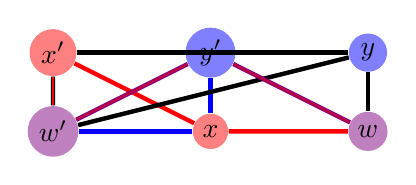
\begin{tikzpicture}[scale=1]
    % Define node styles
    \tikzstyle{red_node} = [circle, fill=red!50, inner sep=2pt]
    \tikzstyle{blue_node} = [circle, fill=blue!50, inner sep=2pt]
    \tikzstyle{purple_node} = [circle, fill=violet!50, inner sep=2pt]

    % Define nodes
    \path node[red_node] (x') at (0, 1) {$x'$}
        node[blue_node] (y') at (2, 1) {$y'$}
        node[blue_node] (y) at (4, 1) {$y$}
        node[purple_node] (w') at (0, 0) {$w'$}
        node[purple_node] (w) at (4, 0) {$w$}
        node[red_node] (x) at (2, 0) {$x$};

    % Draw edges
    \draw[ultra thick, red] (x') -- (x) -- (w);
    \draw[ultra thick, red] (x') -- (y') -- (y);
    \draw[ultra thick, blue] (y') -- (y) -- (w);
    \draw[ultra thick, blue] (y') -- (x) -- (w');
    \draw[ultra thick, black] (x') -- (y) -- (w);
    \draw[ultra thick, black] (x') -- (w') -- (y);
    \draw[ultra thick, violet] (w') -- (y') -- (w);

    % Draw additional edges
    \draw[thick, red] (x') -- (w');
    \draw[thick, purple] (w') -- (y');
    \draw[thick, purple] (y') -- (w);
\end{tikzpicture}

\captionof{figure}{Well-splitting example: Red points are $A-B$, blue points are $B-A$ and violet points are $A\cap B$. $X$ with the semi-coarse space induced by the graph.}
\label{fig:well_splitting_example}
\end{document}